% -*-coding: utf-8;-*-
%%%%%%%%%%%%%%%%%%%%%%%%%%%%%%%%%%%%%%%%%%%%%%%%%%%%%%%%%%%%%%%%%%%%%%%%%%%%%%
% Главный файл
\documentclass[12pt]{rusthesis}
% do not use [draft] otherwise all PS graphics will disappear
\usepackage[T2A]{fontenc}
\usepackage[utf8]{inputenc}
\usepackage{graphicx}
\usepackage{latexcad}
\usepackage{amsmath}
\usepackage{amssymb}
\usepackage{eepic}
\usepackage{epsfig}
\bibliographystyle{plain}

\language=4

% My macros
\newcommand\tablref[1]{\cyrt\cyra\cyrb\cyrl.~\ref{#1}}
\newcommand\figref[1]{\cyrr\cyri\cyrs.~\ref{#1}}
\newcommand\pgref[1]{\cyrs.~\pageref{#1}}
%\newcommand\eqref[1]{(\ref{#1})}

\renewcommand{\tan}{\mathop{\rm tg}}
\renewcommand{\arctan}{\mathop{\rm arctg}}
\renewcommand{\tanh}{\mathop{\rm th}}
\newcommand{\DEF}{\mathrel{\mathop=^{\rm def}}}
\newcommand{\MSE}{\overline{\varepsilon^2}}
\newcommand{\hatMSE}{\overline{\hat{\varepsilon}^2}}
\newcommand{\MSEmin}{\overline{\varepsilon^2}_{\rm min}}
\newcommand{\dt}{\Delta t}
\newcommand{\NN}{\mathcal{N}}
\newcommand{\Emax}{|e|_{max}}

% Activation function
\newcommand{\fa}{\phi}

% Gauss Distribution parameters
\newcommand{\GaDi}[2]{$(#1;#2)$}

% Позволить переносы двух последних букв слова
\righthyphenmin=2

% Дополнительные переносы
\hyphenation{ошиб-ки обыч-но сис-тем не-по-сред-ствен-но-го
ус-пеш-но раз-бро-са раз-брос ав-то-рег-рес-сии од-но-вре-мен-но
не-чет-ко-ло-ги-че-ский
back-pro-pa-ga-tion out-put}

% Нумерация совсем мелких пунктов
\newcounter{subbbcounter}[subsubsection]
\renewcommand{\thesubbbcounter}{%
\arabic{section}.\arabic{subsection}.\arabic{subsubsection}.%
\arabic{subbbcounter}}
\newcommand{\subbbsection}[1]{\par\bigskip\noindent%
\refstepcounter{subbbcounter}%
{\bf\thesubbbcounter.\quad#1}\nopagebreak\smallskip\par}

% Выводы
%\makeatletter
%\newcommand{\l@conclusion}[2]{\noindent\textbf{#1\hfill #2}}
%\newcommand{\conclusion}[1]{\section*{#1}%
%\addcontentsline{toc}{conclusion}{#1}}
%\makeatother

% Russian document tuning in encoding independent format

\renewcommand\contentsname{\CYRO\cyrg\cyrl\cyra\cyrv\cyrl\cyre\cyrn\cyri\cyre}
\renewcommand\listfigurename{\CYRS\cyrp\cyri\cyrs\cyro\cyrk\
  \cyri\cyrl\cyrl\cyryu\cyrs\cyrt\cyrr\cyra\cyrc\cyri\cyrishrt}
\renewcommand\listtablename{\CYRS\cyrp\cyri\cyrs\cyro\cyrk\
  \cyrt\cyra\cyrb\cyrl\cyri\cyrc}
\renewcommand\refname{\CYRL\cyri\cyrt\cyre\cyrr\cyra\cyrt\cyru\cyrr\cyra}
\renewcommand\indexname{\CYRP\cyrr\cyre\cyrd\cyre\cyrt\cyrn\cyrery\cyrishrt\
  \cyru\cyrk\cyra\cyrz\cyra\cyrt\cyre\cyrl\cyrsftsn}
\renewcommand\figurename{\CYRR\cyri\cyrs.}
\renewcommand\tablename{\CYRT\cyra\cyrb\cyrl\cyri\cyrc\cyra}
%\renewcommand\chaptername{\CYRG\cyrl\cyra\cyrv\cyra}
\renewcommand\partname{\CYRCH\cyra\cyrs\cyrt\cyrsftsn}
\renewcommand\appendixname{\CYRP\cyrr\cyri\cyrl\cyro\cyrzh\cyre\cyrn\cyri\cyre}
\renewcommand\abstractname{\CYRA\cyrn\cyrn\cyro\cyrt\cyra\cyrc\cyri\cyrya}
\def\today{\number\day\space\ifcase\month\or
  \CYRYA\cyrn\cyrv\cyra\cyrr\cyrya\or \CYRF\cyre\cyrv\cyrr\cyra\cyrl\cyrya\or
  \CYRM\cyra\cyrr\cyrt\cyra\or \CYRA\cyrp\cyrr\cyre\cyrl\cyrya\or
  \CYRM\cyra\cyrya\or \CYRI\cyryu\cyrn\cyrya\or \CYRI\cyryu\cyrl\cyrya\or
  \CYRA\cyrv\cyrg\cyru\cyrs\cyrt\cyra\or
  \CYRS\cyre\cyrn\cyrt\cyrya\cyrb\cyrb\cyrya\or
  \CYRO\cyrk\cyrt\cyrya\cyrb\cyrr\cyrya\or \CYRN\cyro\cyrya\cyrb\cyrr\cyrya\or
  \CYRD\cyre\cyrk\cyra\cyrb\cyrr\cyrya\fi\space\number\year\space\cyrg.}

%\renewcommand\contentsname{\CYRO\cyrg\cyrl\cyra\cyrv\cyrl\cyre\cyrn\cyri\cyre}
%\renewcommand\listfigurename{\CYRS\cyrp\cyri\cyrs\cyro\cyrk\ \cyrr\cyri\cyrs\cyru\cyrn\cyrk\cyro\cyrv}
%\renewcommand\listtablename{\CYRS\cyrp\cyri\cyrs\cyro\cyrk\ \cyrt\cyra\cyrb\cyrl\cyri\cyrc}
%\renewcommand\bibname{\CYRS\cyrp\cyri\cyrs\cyro\cyrk\ \cyrt\cyra\cyrb\cyrl\cyri\cyrc}
%\renewcommand\indexname{\CYRS\cyrp\cyri\cyrs\cyro\cyrk\ \cyrl\cyri\cyrt\cyre\cyrr\cyra\cyrt\cyru\cyrr\cyrery}
%\renewcommand\figurename{\CYRI\cyrn\cyrd\cyre\cyrk\cyrs\ \CYRR\cyri\cyrs\cyru\cyrn\cyro\cyrk}
%\renewcommand\tablename{\CYRT\cyra\cyrb\cyrl\cyri\cyrc\cyra}
%\renewcommand\partname{\CYRCH\cyra\cyrs\cyrt\cyrsftsn}
%\renewcommand\chaptername{\CYRG\cyrl\cyra\cyrv\cyra}
%\renewcommand\appendixname{\CYRP\cyrr\cyri\cyrl\cyro\cyrzh\cyre\cyrn\cyri\cyre}

% end of file

%%%%%%%%%%%%%%%%%%%%%%%%%%%%%%%%%%%%%%%%%%%%%%%%%%%%%%%%%%%%%%%%%%%%%%%%
% Make section and{sub}section number be with final dot in section title
% and in table of contents but not in \ref.  Autoindent in paragraph
% just after section head.
% Part of latex.ltx is used for this task.  Lines which marked by
% %! . after section number
% are changed comparing with original code.
%
% Usage:
% %%%%%%%%%%%%%%%%%%%%%%%%%%%%%%%%%%%%%%%%%%%%%%%%%%%%%%%%%%%%%%%%%%%%%%%%
% Make section and{sub}section number be with final dot in section title
% and in table of contents but not in \ref.  Autoindent in paragraph
% just after section head.
% Part of latex.ltx is used for this task.  Lines which marked by
% %! . after section number
% are changed comparing with original code.
%
% Usage:
% %%%%%%%%%%%%%%%%%%%%%%%%%%%%%%%%%%%%%%%%%%%%%%%%%%%%%%%%%%%%%%%%%%%%%%%%
% Make section and{sub}section number be with final dot in section title
% and in table of contents but not in \ref.  Autoindent in paragraph
% just after section head.
% Part of latex.ltx is used for this task.  Lines which marked by
% %! . after section number
% are changed comparing with original code.
%
% Usage:
% \input{RusStyle.tex}
% in preambule
%%%%%%%%%%%%%%%%%%%%%%%%%%%%%%%%%%%%%%%%%%%%%%%%%%%%%%%%%%%%%%%%%%%%%%%%
\makeatletter%
\renewcommand\section{\@startsection {section}{1}{\z@}%
                                     {3.5ex \@plus 1ex \@minus .2ex}%
                                     {2.3ex \@plus.2ex}%
                                     {\normalfont\Large\bfseries}}
\renewcommand\subsection{\@startsection{subsection}{2}{\z@}%
                                       {3.25ex\@plus 1ex \@minus .2ex}%
                                       {1.5ex \@plus .2ex}%
                                       {\normalfont\large\bfseries}}
\renewcommand\subsubsection{\@startsection{subsubsection}{3}{\z@}%
                                          {3.25ex\@plus 1ex \@minus .2ex}%
                                          {1.5ex \@plus .2ex}%
                                          {\normalfont\normalsize\bfseries}}
\def\@seccntformat#1{\csname the#1\endcsname.\quad}%! . after section number
\def\@sect#1#2#3#4#5#6[#7]#8{%
  \ifnum #2>\c@secnumdepth
    \let\@svsec\@empty
  \else
    \refstepcounter{#1}%
    \protected@edef\@svsec{\@seccntformat{#1}\relax}%
  \fi
  \@tempskipa #5\relax
  \ifdim \@tempskipa>\z@
    \begingroup
      #6{%
        \@hangfrom{\hskip #3\relax\@svsec}%!
          \interlinepenalty \@M #8\@@par}%
    \endgroup
    \csname #1mark\endcsname{#7}%
    \addcontentsline{toc}{#1}{%
      \ifnum #2>\c@secnumdepth \else
        \protect\numberline{\csname the#1\endcsname.}%! . after section number
      \fi
      #7}%
  \else
    \def\@svsechd{%
      #6{\hskip #3\relax
      \@svsec #8}%
      \csname #1mark\endcsname{#7}%
      \addcontentsline{toc}{#1}{%
        \ifnum #2>\c@secnumdepth \else
          \protect\numberline{\csname the#1\endcsname.}%! . after section number
        \fi
        #7}}%
  \fi
  \@xsect{#5}}
\makeatother%

% in preambule
%%%%%%%%%%%%%%%%%%%%%%%%%%%%%%%%%%%%%%%%%%%%%%%%%%%%%%%%%%%%%%%%%%%%%%%%
\makeatletter%
\renewcommand\section{\@startsection {section}{1}{\z@}%
                                     {3.5ex \@plus 1ex \@minus .2ex}%
                                     {2.3ex \@plus.2ex}%
                                     {\normalfont\Large\bfseries}}
\renewcommand\subsection{\@startsection{subsection}{2}{\z@}%
                                       {3.25ex\@plus 1ex \@minus .2ex}%
                                       {1.5ex \@plus .2ex}%
                                       {\normalfont\large\bfseries}}
\renewcommand\subsubsection{\@startsection{subsubsection}{3}{\z@}%
                                          {3.25ex\@plus 1ex \@minus .2ex}%
                                          {1.5ex \@plus .2ex}%
                                          {\normalfont\normalsize\bfseries}}
\def\@seccntformat#1{\csname the#1\endcsname.\quad}%! . after section number
\def\@sect#1#2#3#4#5#6[#7]#8{%
  \ifnum #2>\c@secnumdepth
    \let\@svsec\@empty
  \else
    \refstepcounter{#1}%
    \protected@edef\@svsec{\@seccntformat{#1}\relax}%
  \fi
  \@tempskipa #5\relax
  \ifdim \@tempskipa>\z@
    \begingroup
      #6{%
        \@hangfrom{\hskip #3\relax\@svsec}%!
          \interlinepenalty \@M #8\@@par}%
    \endgroup
    \csname #1mark\endcsname{#7}%
    \addcontentsline{toc}{#1}{%
      \ifnum #2>\c@secnumdepth \else
        \protect\numberline{\csname the#1\endcsname.}%! . after section number
      \fi
      #7}%
  \else
    \def\@svsechd{%
      #6{\hskip #3\relax
      \@svsec #8}%
      \csname #1mark\endcsname{#7}%
      \addcontentsline{toc}{#1}{%
        \ifnum #2>\c@secnumdepth \else
          \protect\numberline{\csname the#1\endcsname.}%! . after section number
        \fi
        #7}}%
  \fi
  \@xsect{#5}}
\makeatother%

% in preambule
%%%%%%%%%%%%%%%%%%%%%%%%%%%%%%%%%%%%%%%%%%%%%%%%%%%%%%%%%%%%%%%%%%%%%%%%
\makeatletter%
\renewcommand\section{\@startsection {section}{1}{\z@}%
                                     {3.5ex \@plus 1ex \@minus .2ex}%
                                     {2.3ex \@plus.2ex}%
                                     {\normalfont\Large\bfseries}}
\renewcommand\subsection{\@startsection{subsection}{2}{\z@}%
                                       {3.25ex\@plus 1ex \@minus .2ex}%
                                       {1.5ex \@plus .2ex}%
                                       {\normalfont\large\bfseries}}
\renewcommand\subsubsection{\@startsection{subsubsection}{3}{\z@}%
                                          {3.25ex\@plus 1ex \@minus .2ex}%
                                          {1.5ex \@plus .2ex}%
                                          {\normalfont\normalsize\bfseries}}
\def\@seccntformat#1{\csname the#1\endcsname.\quad}%! . after section number
\def\@sect#1#2#3#4#5#6[#7]#8{%
  \ifnum #2>\c@secnumdepth
    \let\@svsec\@empty
  \else
    \refstepcounter{#1}%
    \protected@edef\@svsec{\@seccntformat{#1}\relax}%
  \fi
  \@tempskipa #5\relax
  \ifdim \@tempskipa>\z@
    \begingroup
      #6{%
        \@hangfrom{\hskip #3\relax\@svsec}%!
          \interlinepenalty \@M #8\@@par}%
    \endgroup
    \csname #1mark\endcsname{#7}%
    \addcontentsline{toc}{#1}{%
      \ifnum #2>\c@secnumdepth \else
        \protect\numberline{\csname the#1\endcsname.}%! . after section number
      \fi
      #7}%
  \else
    \def\@svsechd{%
      #6{\hskip #3\relax
      \@svsec #8}%
      \csname #1mark\endcsname{#7}%
      \addcontentsline{toc}{#1}{%
        \ifnum #2>\c@secnumdepth \else
          \protect\numberline{\csname the#1\endcsname.}%! . after section number
        \fi
        #7}}%
  \fi
  \@xsect{#5}}
\makeatother%


\input{txdtools.tex}
\input{blockdiagram.tex}

% Для макросов texdraw установить умолчательной единицей измерения миллиметры
%texdraw \everytexdraw{\drawdim mm}

\title{Стохастический квазиоптимальный нейросетевой регулятор}

\author{Елисеев Владимир Леонидович}

\begin{document}

% Титульные страницы
%\maketitle

% Оглавление
\setcounter{tocdepth}{4}\tableofcontents
%\newpage

% Введение
\chapter*{Введение}
\addcontentsline{toc}{chapter}{Введение}

%% -*-coding: utf-8;-*-
%%%%%%%%%%%%%%%%%%%%%%%%%%%%%%%%%%%%%%%%%%%%%%%%%%%%%%%%%%%%%%%%%
% Введение

\paragraph{Актуальность работы}
Актуальность данной работы обусловлена всё более широким
использованием искусственных нейронных сетей (ИНС) в различных
областях науки и техники.  При этом одним из важных направлений их
использования являются системы автоматического управления различных
типов.  Известны примеры успешного нейросетевого решения модельных
задач, таких как управления обратным маятником.  Нейронные сети на
практике используются в робототехнике для управления манипуляторами и
мобильными устройствами, в промышленности с непрерывными
производственными процессами разных типов, в атомной энергетике для
идентификации и управления переходными процессами.

Все это требует проведения теоретических и практических исследований
нейронных сетей, особенностей их применения в системах управления, а
также сопоставления с другими подходами.  С этим же связана и задача
совершенствования соответствующего научно-методического обеспечения,
развития средств анализа и моделирования систем нейросетевого
управления.

Работы по данной проблеме велись и ведутся весьма интенсивно как
отечественными (А.~И.~Галушкин, В.~А.~Терехов, А.~Н.~Горбань,
В.~И.~Комашинский, Д.~А.~Смирнов, Т.~А.~Бондарь, А.~С.~Логовский и
др.). Тем не менее многие вопросы либо исследованы недостаточно полно,
либо ориентированы на решение относительно узких прикладных задач.  В
частности, отсутствуют работы, посвященные систематизации замены
традиционного регулятора на нейросетевой, обобщающие накопленный к
настоящему времени опыт применения последних.  Нет публикаций, в
которых сопоставляется нейросетевое и линейное управление при
использовании общего среднеквадратического критерия оптимальности.
Достаточно ограничен перечень работ по нейросетевому управлению
нестационарным объектом.  Всё это свидетельствует о необходимости
дальнейшего развития исследований по данной проблематике.

\paragraph{Цель исследований}
Целью диссертационной работы развитие методов и алгоритмов
нейросетевого управления с акцентом на систематизацию предлагаемых
подходов.  В частности, представляется важным рассмотреть вопросы
выбора структуры входов и архитектуры нейронных сетей, влияния
исходных данных на настройку нейронной сети, сформулировать
обоснованные с точки зрения практического применения процедуры
обучения нейросетевых регуляторов в контуре управления и вне его как в
случае неизменных условий, так с нестационарным объектом.

В соответствии с указанной целью в рамках диссертационной работы
поставлены и решались следующие задачи:
\begin{enumerate}
\item
Обзор и анализ известных подходов применения ИНС в системах
управления, используемых методов и программных средств.

\item
Разработка методики синтеза нейросетевого регулятора – аналога П, ПИ и
ПИД регуляторов и сопоставление их свойств.

\item
Исследование возможностей нейросетевого подхода при построении САУ по
критерию минимума среднеквадратической ошибки.

\item 
Развитие нейросетевых алгоритмов управления нестационарными объектами.

\item
Применение полученных методических, математических и
программно-алгоритмических результатов при решении практических задач
управления подвижным роботом и в учебном процессе.
\end{enumerate}

\paragraph{Методы исследования}
Полученные результаты исследования базируются на использовании методов
и средств системного анализа, теории искусственных нейронных сетей и
теории автоматического управления, математической статистики,
имитационного моделирования.

\paragraph{Защищаемые научные положения и их новизна}

\begin{enumerate}
\item 
Методика синтеза нейросетевого регулятора --- аналога П, ПИ и ПИД
регуляторов, --- включающая в себя выбор структуры входов и внутренней
архитектуры используемой ИНС, оптимальное формирование обучающей
выборки, проведение обучения ИНС, обеспечивающая замену исходного
регулятора на нейросетевой без потери качества управления.

\item
Способ построения и настройки нейросетевого регулятора по критерию
минимума среднеквадратической ошибки и доказательство его
эффективности в стандартных условиях и робастности при изменении
параметров объекта управления.

\item
Алгоритм управления нестационарным объектом на основе комбинированного
использования нейросетевого и статистического подходов.

\item
Нейросетевой алгоритм управления мобильным роботом для движения на маяк.

\item
Программно-алгоритмический комплекс имитационного моделирования и
исследования нейросетевых систем управления, обеспечивающий реализацию
предлагаемых в работе методов и сопоставление нейросетевых алгоритмов
управления с традиционными, а также удобный для использования в
учебном процессе.
\end{enumerate}


\paragraph{Обоснованность и достоверность научных положений, выводов
и рекомендаций} подтверждаются корректным использованием методов
теории искусственных нейронных сетей и теории автоматического
управления, результатами имитационного моделирования и практического
использования разработанных методов, алгоритмов и прикладных программ.

\paragraph{Научная значимость работы} состоит в разработке научно
обоснованной методики замены ПИД регулятора на нейросетевой,
исследовании нейросетевого алгоритма оптимального управления и его
сравнительного анализа с винеровским оптимальным регулятором,
расширении метода нейросетевого управления на случай нестационарного
объекта с использованием алгоритма кумулятивных сумм, систематизации и
решении ряда вопросов, возникающих при обучения нейронных сетей в роли
регулятора и модели объекта управления.

\paragraph{Практическая значимость работы}
Результаты исследований, выполненных в диссертационной работе, были
использованы при синтезе нейросетевого алгоритма управления подвижным
роботом и опробованы на практике.  Разработанный подход позволяет
легко адаптировать нейросетевой алгоритм для управления широким
классом мобильных устройств с различными массо-габаритными
характеристиками и динамическими свойствами без применения
аналитической идентификации параметров устройства.  Созданные
алгоритмы легли в основу программного комплекса моделирования
нейросетевых систем управления, который может использоваться для
синтеза и исследования нейросетевых алгоритмов управления и их
сравнения с альтернативными подходами.  Данный комплекс является
интерактивным, модульным, легко расширяется под специфические задачи и
адаптирован для применения в учебном процессе в качестве программного
стенда для проведения лабораторных работ.

\paragraph{Реализация результатов}

Результаты работы были использованы:
\begin{itemize}
\item
для разработки алгоритма нейросетевого управления автономным мобильным
роботом в Московском государственном техническом университете
им. Н.~Э.~Баумана;
\item
при создании учебно-практического лабораторного комплекса по курсу
``Нейрокомпьютеры и их применение'' в Московском энергетическом
институте (техническоом университете).
\end{itemize}

\paragraph{Апробация работы} Результаты работы и ее основные положения
докладывались на XXXV Международной конференции ``Информационные
технологии в науке, образовании, телекоммуникации, бизнесе'' –
IT+SE’2008 (Ялта-Гурзуф, 2008г.), ``Информационные средства и
технологии'' (Москва, 1999~г., 2000~г.), ``Актуальные проблемы защиты
и безопасности'' (Санкт-Петербург, 2006~г.), ``International
Scientific Colloquium'' (Ильменау, Германия, 2000~г., 2010~г.), на
заседании кафедры ``Управление и информатика'' Московского
энергетического института (технического университета).

\paragraph{Публикации}
По результатам исследований опубликовано 11 научных
работ~\cite{elfil-pta99,
filelav-ict99,filel-ict2000,filel-ist2000,elfil-iwk2000,filel-ict2003,
el-neurocomp2002,elzenk-extrob2006,elfil-modctrl2006,filel-iwk2010,
elfil-vestmei2010}.

\paragraph{Структура и объем работы}
Диссертационная работа состоит из введения, шести глав, заключения и
списка литературы из 79 наименований, включает 162 страницы текста, ???
рисунков, ??? таблиц.

\paragraph{Краткий обзор глав}

% Глава 1

В первой главе делается обзор прикладных областей, в которых активно
исследуются вопросы применения нейронных сетей в системах управления.
Дается краткий анализ причин актуальности этих исследований.

Рассматриваются основные архитектуры нейронных сетей, применяемые в
системах управления.  Описывается их устройство и проводится
классификация по способу реализации динамических свойств.
Перечисляются базовые и усовершенствованные алгоритмы обучения.
Формулируются типичные вопросы, возникающие при проектировании
нейросети для решения конкретной прикладной задачи.

На основе анализа литературы перечисляются основные способы применения
нейронных сетей в системах управления.  Подробно рассматриваются и
анализируются различные подходы к синтезу нейросетевого регулятора.
Описываются основные схемы обучения, применяемые исследователями, и их
свойства.  Далее делается обзор методов нейросетевой идентификации и
их сопоставление с методами линейной идентификации.  Приводятся схемы
реализации нейросетевых моделей и отмечаются характерные особенности
при их синтезе и эксплуатации.  В отдельную группу выделены прочие
способы использования потенциала нейронных сетей.  Сюда отнесены
гибридные регуляторы, нейросети--настройщики регуляторов иных типов и
алгоритмы нейросетевой фильтрации.

Подчеркивается важность проведения систематического сопоставления
традиционных линейных и нейросетевых регуляторов, а также выявления
отличительных свойств последних.  Анализируются публикации по данной
тематике.  Отмечается целесообразность сопоставления как с наиболее
распространенным ПИД регулятором по причине высокой практической
ценности такого исследования, так и с винеровским оптимальным
регулятором по причине эквивалентности постановки задачи синтеза, что
делает сопоставление максимально корректным.

Рассматриваются основые задачи, возникающие при изучении нейронных
сетей в системах управления.  Отмечается неполнота их реализации в
основных пакетах универсального и нейросетевого моделирования.
Отдельно рассматриваются online-ресурсы, используемые для демонстрации
нейросетевых алгоритмов.  Отмечаются их недостатки с точки зрения
исследователя и преподавателя высшей школы.  Делается вывод об
актуальности разработки программного пакета, совмещающего в себе
возможности моделирования САУ и обучения нейронных сетей для решения
задач управления с целью использования в учебном процессе.

% Глава 2

Во второй главе формулируется задача замены ПИД регулятора на
нейросетевой с позиции аппроксимации функции ПИД регулятора нейросетью
вне контура управления по критерию минимизации среднеквадратической
ошибки имитации.  Определяются основные этапы методики синтеза
нейросетевого регулятора (НС--Р), среди которых выбор архитектуры
нейросети, сбор обучающих данных, обучение, проверка качества имитации
и функционирования.

Далее рассматривается вопрос выбора архитектуры нейросети регулятора.
Под архитектурой понимается совокупность набора входов для реализации
динамических свойств, количества слоев сети и распределения нейронов в
них.  Последовательно рассматриваются варианты компонентов архитектуры
и в рамках имитационных экспериментов выявляются наиболее приемлемые
из них.

Проводится исследование о влиянии вида пробного сигнала, используемого
для получения обучающей выборки, на качество имитации НС--Р.
Последующий анализ позволяет сформулировать основной критерий,
обеспечивающий качество результирующего нейросетевого регулятора ---
степень равномерности распределения облака обучающих точек в
многомерном пространстве области определения функции аппроксимации.
Достижение минимальной плотности покрытия области определения дает
необходимую длину обучающей выборки.

Приводится алгоритм пакетного обучения НС--Р методом обратного
распространения ошибки.  Обсуждаются вопросы выбора коэффициента
скорости обучения и критерия останова, а также контроля за обобщающей
способностью сети в процессе обучения.  Приводятся эвристические
решения этих вопросов, успешно используемые автором в вычислительных
экспериментах.  Отмечается неэквивалентность качества имитации
исходного регулятора вне контура управления и в нём.

В качестве примера сформулированной методики синтеза рассматривается
задача управления температурой в химическом реакторе непрерывного
действия с мешалкой.  Объект управления является существенно
нелинейным и управляется ПИД регулятором.  Последовательно применяя
рекомендации методики, синтезируется нейросетевой регулятор,
обеспечивающий качество управления не хуже исходного.  Отмечается
важность выбора подходящей архитектуры НС--Р.  Анализируются свойства
полученного нейросетевого регулятора по сравнению с ПИД.

% Глава 3

В третьей главе формулируется задача синтеза нейросетевого
оптимального регулятора в постановке, аналогичной винеровской
фильтрации.  Отмечается важность формирования эталона для обучения
нейросетевого регулятора с помощью инверсии объекта управления.

Обосновывается необходимость использования нейросетевой модели объекта
управления и показывается, как такая модель может использоваться для
получения эталонного управляющего воздействия используя аппарат
обратного распространения.  Эта модель должна функционировать в
контуре управления одновременно с регулятором в процессе его обучения.
Подчеркивается связь функций нейронной сети модели в прямом и в
обратном направлениях с якобианом объекта управления.

Обсуждается методика синтеза нейросетевой модели предсказания
поведения объекта управления вне контура.  Такая модель не является
автономной, то есть, ей необходим объект управления.  Однако её синтез
значительно проще автономных моделей, применимость для обучения
нейросетевого регулятора ничем не хуже.  На основе результатов,
полученных в имитационных экспериментах выясняются значимые и
незначимые параметры архитектуры нейронной сети модели, а также их
связь с параметрами объекта управления.

Далее исследуется вопрос формирования обучающей и тестовой выборок
экспериментальных данных для целей построения качественной
нейросетевой модели.  Рассматриваются типовые пробные сигналы
(ступенчатый, гармонический и стохастический) и их влияние на качество
получающейся модели.  Вводятся понятия области гарантированного
качества и надежности по амплитуде, на основе которых сравниваются
пробные сигналы.  Для стохастического пробного сигнала исследовано
влияние реализации выборки на обучение нейросетевой модели разных
архитектур.

Для исследования алгоритма обучения нейросетевого оптимального
регулятора вводится понятие идеальных условий, реализуемых только в
рамках имитационного эксперимента, когда каждый цикл обучения (эпоху)
повторяются одинаковые выборки уставки и помехи.  В идельных условиях
проводится ряд экспериментов, дающих ответы на вопросы о влиянии
сложности архитектуры нейросетевой модели, коэффициента скорости
обучения и длительности эпохи на процесс обучения нейросетевого
оптимального регулятора.

При обучении нейросетевого оптимального регулятора в реальных услових
проводятся исследования поведения среднеквадратической ошибки
управления и идентификации в процессе обучения, и о влиянии начального
приближения на процесс обучения и его результат.  Ставится задача
определения момента завершения обучения нейросетевого регулятора.  Для
обоснования метода решения используются результаты, полученные в
идеальных условиях.

Учитывая очевидную аналогию полученного нейросетевого и винеровского
оптимального регуляторов, проводится их сопоставление.  В частности, в
имитационных экспериментах исследуется вопрос качества управления в
номинальных и отличающихся условиях по уставке.  Это позволяет сделать
вывод о большей робастности нейросетевого оптимального регулятора по
сравнению с винеровским.

% Глава 4

В четвертой главе рассматривается задача нейросетевого управления
нестационарным объектом.  Отмечается её важность и актуальность.  В
качестве модели нестационарности для дальнейших исследований
используется ступенчатое изменение параметров объекта.

Предлагаются два альтернативных варианта адаптации нейросетевого
регулятора к изменению параметров объекта: постоянная адаптация с
постоянной подстройкой модели объекта и адаптация по обнаружению
разладки.  Оба подхода основаны на методе синтеза нейросетевого
оптимального регулятора, описанного в третьей главе, однако первый
использует только нейросетевые алгоритмы, а второй использует также
алгоритм кумулятивных сумм, используемый для обнаружения момента
изменения параметров объекта.

Приводятся схемы применения обоих вариантов и отмечаются особенности
использования в них нейросетевых моделей.  В частности, в методе с
обнаружением разладки нейросетевая модель используется для получения
ошибки идентификации, анализируемой алгоритмом кумулятивных сумм
(АКС).  После успешной диагностики разладки модель объекта
подстраивается вне контура управления к новым динамическим свойствам
объекта и далее используется в контуре для обучения нейросетевого
регулятора.

Отмечается важность задания параметров АКС для достижения желаемых
величин среднего времени между ложными тревогами и среднего времени
запаздывания.  Приводятся графики зависимости этих параметров от
выбранного порога для одного из имитационных экспериментов.

Ключевым моментом любого алгоритма управления нестационарным объектом
является его полная автоматизация, что позволяет исключить
человеческий фактор, увеличив надежность САУ и её эффективность.  Для
достижения этой цели представлена методика автоматического
формирования обучающей выборки для настройки модели объекта.

В сравнительных экспериментах исследуются свойства обоих предложенных
методов как в нестационарных, так и в стационарных условиях,
отмечаются их достоинства и недостатки.

% Глава 5

В пятой главе рассматривается задача нейросетевого управления
мобильным колесным роботом.  Описывается конструкция робота и основные
элементы системы управления.  Формулируется задача управления роботом
при прямолинейном движении на маяк и подчеркивается её базовый
характер для решения других задач управления движением по более
сложным траекториям.  При отсутствии информации о дистанции до маяка
отмечается эквивалентность задачи поддержания точного направления на
маяк задаче минимизации ошибки движения по траектории.

Предлагается применение методик построения нейросетевой имитации
исходного регулятора и синтеза нейросетевого оптимального регулятора,
изложенных в главах 2 и 3, для управления мобильным роботом.  В синтез
проводится в соответствии с разработанными методиками.
Демонстрируются данные реальных экспериментов с роботом.  Отмечается
работоспособность предложенных методик и существенный рост качества
управления по сравнению с исходным регулятором.

% Глава 6

В шестой главе описывается разработанный программный пакет для
изучения искусственных нейронных сетей в системах автоматического
управления.  Пакет позволяет последовательно реализовать методики
нейросетевого управления, описанные в главах 2--4.  Отмечается
важность и актуальность этого пакета для образовательных и
исследовательских целей.

Перечисляются основные характеристики пакета, решаемые в нём задачи и
основные функции.  Описывается структура пакета и используемые
инструментальные средства: языки {\tt C++} и {\tt tcl/tk}.
Описывается структура пакета, его интерактивная и вычислительная
части.  Также приводятся описания форматов используемых файлов.
Раскрываются возможности пакета по представлению нейронных сетей,
моделированию линейных и нелинейных звеньев, способ задания
нестационарных элементов САУ, а также метод моделирования САУ в целом
с помощью сетей Петри.

Далее описывается принцип применения пакета в курсе лабораторных
работ, посвященных изучению нейросетевых алгоритмов управления.
Освещаются дидактические аспекты и способ интеграции лабоработных в
учебный процесс.

Приводится описание трех лабораторных работ по темам: синтез
нейросетевого оптимального регулятора; сравнительный анализ
нейросетевого, винеровского и ПИД регуляторов; нейросетевое управление
нестационарным объектом.  По каждой лабораторной работе приводятся
цель, постановка задачи, план работы, а также возможные варианты.
Приводятся примеры отчетов по лабораторным работам.

%\paragraph{Указание на наличие приложений}


% Глава 1
\chapter{Обзор применения нейронных сетей в задачах автоматического управления}
%\input{part_review.tex}

% Глава 2
\chapter{Метод синтеза нейросетевого оптимального регулятора}
%\input{part_noc_synthesis.tex}

% Глава 3
\chapter{Выбор архитектуры нейронных сетей и параметров их обучения}
%\input{part_nn_arch_and_params.tex}

% Глава 4
\chapter{Сравнительный анализ нейросетевого оптимального, ПИД и винеровского регуляторов}
%\input{part_compare_controllers.tex}

% Глава 5
\chapter{Нейросетевое управление в нестационарных условиях}
%\input{part_non_steady_conditions.tex}

% Глава 6
\chapter{Нейросетевое управление мобильным роботом}
%\input{part_mobile_robot.tex}

% Глава 7
\chapter{Программный комплекс для обучения методам нейросетевого управления в учебном процессе}
% -*-coding: utf-8;-*-
%%%%%%%%%%%%%%%%%%%%%%%%%%%%%%%%%%%%%%%%%%%%%%%%%%%%%%%%%%%%%%%%%%%%%%%%%%%%%%
% Программный комплекс для обучения методам нейросетевого управления в
% учебном процессе

\section{Цель работы}


Разработка интерактивного программного комплекса для настройки и
моделирования традиционных и нейросетевых систем управления с обратной
связью.

Преподавание нейросетевых методов на инженерных специальностях должно учитывать специфику 


\subsection{Мотивация}

Искусственные нейронные сети представляют собой относительно новый
мощный и многогранный инструмент для решения разнообразных инженерных
и научно-исследовательских задач.  Способ применения нейронных сетей
достаточно специфичен, так как он основан не на аналитическом
формализме, а на обучении --- неявном извлечении взаимосвязей из
представленных данных.  Эта особенность отличает нейросетевые методы
от традиционных в том числе и в задачах автоматического управления.

Аналитические методы давно и прочно укоренились в учебных курсах на
инженерных специальностях.  Для освоения аппарата этих методов
студентам предлагается большое количество разнообразных упражнений,
суть которых сводится к аналитическому решению задачи, то есть, к
выводу формальным способом решения в общем виде.  Только в том случае,
если математический аппарат не позволяет получить чточное решение в
аналитической форме, используются приближенные способы решения, в том
числе, с помощью численных методов.  Однако в любом случае вид
решения, а значит и его свойства, определяются человеком.

Нейросетевые методы подразумевают участие человека только в
обеспечении процесса обучения, а собственно решение формируется
нейросетью само.  Его вид и свойства изначально неизвестны.  Более
того, после успешного завершения обучения нейронной сетью, отличной от
тривиальной, человеку практически невозможно понять, какие решения
приняла сеть и и как это повлияло на достижение поставленной цели.
Иногда даже говорят о самостоятельной задаче извлечения знаний из
обучечнной нейронной сети.

Написать про неполноту формального описания ИНС.

Изложенные особенности свидетельствуют об особой важности практических
работ в учебном курсе по нейросетевым методам.  Только они дают
возможность студентам увидеть, как происходит процесс обучения и как
функционирует обученная нейронная сеть в рамках решения конкретной
прикладной задачи.  Это невозможно до конца формализовать на лекциях и
изложить в учебных пособиях.  Фактически, совокупность архитектуры НС,
метода обучения с его параметрами, а также обучающих данных дает
уникальное решение, выражающееся в наборе весовых коэффициентов НС.

Обычно для практических работ по курсу искусственных нейронных сетей
используется тот или иной универсальный (Statistica, MatLab, Octave)
или специализированный нейросетевой (Stuttgart Neural Network
Simulator, Neural Lab, Trajan) программный пакет.  Для большинства
типовых задач, решаемых с помощью НС (распознавание образов,
ассоциативная память, кластеризация и т.п.), возможностей
перечисленных пакетов вполне достаточно.  К ним относятся:

\begin{itemize}
\item Задание архитектуры нейросети и метода её обучения
\item Задание обучающего множества
\item Задание параметров обучения
\item Обучение нейронной сети
\item Анализ качества работы обученной нейронной сети
\end{itemize}

Однако применение НС в задачах управления требует дополнительно
наличия многих функций, отсутствующих в пакетах нейросетевого
моделирования:

\begin{itemize}
\item Задание вида и параметров регулятора и объекта управления
\item Задание входных сигналов - уставки и помехи
\item Съем данных из различных точек контура управления для
  визуализации и обучения НС
\item Моделирование САУ
\item Сравнение и анализ качества работы САУ с различными
  компонентами, в том числе, с нейросетевыми
\end{itemize}

В универсальных же пакетах (класса MatLab) реализация перечисленных
функций требует достаточно серьезного программирования как
вычислительных, так и интерактивных и графических функций.  В то же
время, получающаяся программа обладала бы ограниченным
быстродействием, так как должна быть написана на интерпретируемом
языке программирования.  Вопросы быстродействия в данном классе задач
достаточно важны, так как моделирование и обучение нейронных сетей
производится на длинных временных рядах (порядка $10^4 ... 10^6$
отсчетов).

Представляется актуальным разработать интерактивный пакет программ,
позволяющий решать задачи нейросетевого управления и сопоставлять
нейросетевые подходы с традиционными.  На базе такого пакета можно
создать курс практических занятий для студентов инженерных
специальностей, изучающих применение нейронных сетей в системах
автоматического управления.  Подобный программный комплекс был бы
полезен и для исследовательских проектов, позволяя быстро провести
моделирование проектируемой САУ и оценить возможности использования в
ней нейросетевого управления.


\section{Постановка задачи}
Фактически, Т.З. на три лабораторных работы:
\begin{itemize}
\item Синтез нейросетевого регулятора
\item Сравнительный анализ нейросетевого, винеровского и ПИД регуляторов
\item Управление нестационарным объектом
\end{itemize}

Совершенствование лабораторной базы.  Предлагается создать лабораторные работы.

Программный комплекс.
Задачи, возложенные на этот комплекс.

\subsection{Структура комплекса}
\subsection{Принципы взаимодействия}

\subsection{Дидактические цели}
Что должен знать и уметь студент по результатам выполнения лабораторных работ.

\subsection{План методички}
\begin{itemize}
\item Введение: цель работы
\item Теоретическая часть - взять из 2, 3, 4 глав
\item Задание на выполнение работы
\item Инструкция по проведению работы (описание программного комплекса)
\item Представление результатов
\item Контрольные вопросы
\end{itemize}

\section{Методическая база}
\subsection{Примеры отчетов - в приложении}


% Заключение
\chapter*{Заключение}
\addcontentsline{toc}{chapter}{Заключение}

% Библиография
\bibliography{Bibliogr}

% Приложения
%\appendix

% Приложение 1 - Эксперименты
%\section{Сравнительные эксперименты с ПИД, Винеровским и нейросетевым
%         оптимальными регуляторами}
%% -*-coding: koi8-r;-*-
% ���������� 1 - ������������ �� ������������ ��������������� ����������
% � ������������ ������

%%%%%%%%%%%%%%%%%%%%%%%%%%%%%%%%%%%%%%%%%%%%%%%%%%%%%%%%%%%%%%%%%

� ��������� ���������� ���������� ��������� �������� ������������� �
�� ����������.  � ������������� ��������� ������� ���, �����������
����������� � ������������ ����������� ����������.  ���� �������������
����������� � ��������� ������������ ������������� ��\-����������
���������� � �������� ������������ ������ �� ��������� � �������������
���������� ��������� ����������.\label{appendix1}

����������� ��������� �������� �� ���� ������������� ������ ����
�����������.  ����������� ������ ��������� ������� --- �����������
����� 1-�� �������.  ������� ������ ��� ����� ��� ���������
������������ ���������.  ������� ������ ��������� ������� � ���, ���,
��-������, ��� ������ ����� ������������ �� �������� ��� ����������
����������� � ������� ��� �������������, ��-������, � ����� �������
������� ��������� ��� ������������ ������������ ������� ����������
���������� ����������, ��� � ������������ ������� ��������� ���
���������� ����������.

��������� ��� ���������� ����������� �������� � ����������� ��
����������� ������� ��� ���������� ������.  ������������� ���������
���������� ���� ��������� �� ������ ������������� ������������, �
������������ ��������������� ��� ������� �� ��������� � ���
�������������.

������ ������������ ���������� ���������� ������������.
��������������� ��������� ��������, ����� ��������� �������� � �������
���������� �������� �����.  � ���������� ��������� ����� ������� �
��������� ������������.  ����� ����, ��� ������� � ������� ������
���������� ������������� ������������� ������, ��� ��� �������.
�������, �������� ����������� ������� �������������, � �������������
�������������� ������� ������� � ������� ����������.

������ ������������� ������������ ���������� (���) ���������� �
����������� �������� ��� ������������� ��������� ���������� ��
��������, ���������� � �.\ref{noc_synthesis_method}.

\section{������ ���������� ������� �������}
% ������ ���������� ������� �������
\label{W1op_case}

�������, ���������������� �������� ����������� ������, ��������
���������� ��������� �� ������ �������� �������� ����������.  �
���������, ����� ����� ������� ������� � ������������ ��� ���������
������������� ������ ������������� �������� ����������� �������.

\subsection{����������� �������}%
\label{W1op_nominal_cond}

\begin{itemize}

\item
����������� ������ �������:
$R^*_1(z)=\mathcal{Z}\Bigl\{\displaystyle\frac{2.5}{1+4s}\Bigr\}
         =\displaystyle\frac{0.625z}{z-0.7788}$

\item
����������� ������ ������:
$N^*_1(z)=0.1$

\item
����������� ����������� ������:
$W^*_1(z)=\displaystyle\frac{0.9754z}{z-0.0192}$

������������������ ������ ���������� $\MSE_{min}=0.0098$

\item
������ ����������:
$P^*_1(z)=\displaystyle\frac{3z}{z-0.8}$

\item
����������� ����������� ���������:
$C^*_{WOC_1}=\displaystyle\frac{0.3251z-0.2601}{z-0.9946}$

\item
�������� ��� ��������� (��. \figref{fig:dw1op_pid_step}):
$$
C^*_{PID_1}(z)=0.2 +
             0.08\displaystyle\frac{z}{z-1} +
             0.05\displaystyle\frac{z^2-2z+1}{z(z-1)}
$$

\end{itemize}

\begin{figure}[h]
\centering
\hbox{\psfig{figure=dw1op_pid_step.ps,angle=270,width=0.8\textwidth,%
             height=0.35\textheight}}
\caption{���������� �������������� ���������� ������� ��� ��� ����������.}
\label{fig:dw1op_pid_step}
\end{figure}

\subsection{����������� � ��������� �������� ��--�}%
\label{W1op_NNP_descr}

\begin{itemize}

\item
����������� ��--�: $\NN^o_{1+1,1}$

\item
������������ �������� ��������: $\eta_h=0.01$, $\eta_o=0.001$

\item
��������� �������: ����� $L=1000$, ��������� �������� ��������:
$u=[-0.80, 0.80]$, $y=[-2.89, 3.88]$
%$u=[-0.7997, 0.8008]$, $y=[-2.8877, 3.8840]$

\item
����������� �������: ����� $L=1000$, ��������� �������� ��������:
$u=[-0.80, 0.72]$, $y=[-4.02, 4.16]$
%$u=[-0.8010, 0.7169]$, $y=[-4.0234, 4.1574]$

\item
�������� � ������� 95 ���� �� ������ ����� $\MSE$ �� ����������� �������.

\end{itemize}

\subsection{����������� � ��������� ���������������� �������� ��--�}%
\label{W1op_NNCpre_descr}

\begin{itemize}

\item
����������� ��--P: $\NN^o_{1+1,1}$

\item
������������ �������� ��������: $\eta_h=0.05$, $\eta_o=0.005$

\item
��������� �������: ����� $L=500$, ��������� �������� ��������:
$r=[-2.62, 2.59]$, $e=[-1.94, 1.73]$, $u=[-0.66, 0.58]$
%$r=[-2.6234, 2.5899]$, $e=[-1.9396, 1.7348]$, $u=[-0.6638, 0.5822]$

\item
����������� �������: ����� $L=500$, ��������� �������� ��������:
$r=[-2.58, 3.22]$, $e=[-2.25, 2.09]$, $u=[-0.67, 0.80]$
%$r=[-2.5778, 3.2184]$, $e=[-2.2461, 2.0882]$, $u=[-0.6730, 0.7979]$

\item
�������� � ������� 10 ���� �� �������� �������� ���������� ������ ��
����������� ������� ������ $10^{-5}$.

\end{itemize}

\subsection{��������� ���������� ��--� � �������}%
\label{W1op_NNCfin_descr}

\begin{itemize}

\item
������������ �������� ��������: $\eta_h=0.0001$, $\eta_o=0.00005$

\item
������������ ����� $L=300$

\item
�������� �������� � ����������� �������� �������� $\MSE$
�������������� �� ���� 50 ����.  ��� �������� �������������
������������ �������� �����, ���������� �� �������
(\cite[�.~797--799]{aivmhit98}).  ������� ���������� ��������
$\alpha=5\%$.

\item
�������� ����������� �������� �������� $\MSE$ ��������� �������� ��
����� �� ����� ����, �� ����, �������� ���� ����������� ����� 250
��������� ����.

\end{itemize}

\subsection{������������� �������}%
\label{W1op_differ_cond}

\begin{description}

\item[$E_{r-}$:]
����������� �������� �������: $R^*_1(z)=\displaystyle\frac{0.313z}{z-0.7788}$

\item[$E_{r+}$:]
����������� �������� �������: $R^*_1(z)=\displaystyle\frac{1.250z}{z-0.7788}$

\item[$E_{n-}$:]
����������� �������� ������: $N^*_1(z)=0.05$

\item[$E_{n+}$:]
����������� �������� ������: $N^*_1(z)=0.2$

\item[$E_m$:]
������� ������������ ����� ������������������ ������������� ���������
���������� 1, �������� 40 � ������������� �������� 20 ����������
�������� �������.  ����� ����� ���������� ���� ��������� 150
���������� �������� �������.

\item[$E_s$:]
������� ������������ ����� ������������� ������ ��������� 1 � ��������
�������.  ��� ������������ �������� ���������� �� ��������� ��������
���� ��������� ������������ � �������� �������������� ������� �� 2 ��
50 ���������� �������� �������.  ����� ����� ���������� ���� ����
����� 500 ���������� �������� �������.  ������������ ����������� �
������� ������� ��� ����, ����� �������� ��������� ��� �����������
�������� ���������� �� �������.

\item[$E_p$:]
������ ���������� � ����������� �� ��������� � �����������
��������������: $P^*_{1'}(z)=\displaystyle\frac{3z}{z-0.4}$

\end{description}

\subsection{���������� �������������}%
\label{W1op_results}

���������� ������������ �� ����� � ��� �� ������������ ������� �������
� ������.  ����� ��������� ���������� ���� ���������� 10000 ����������
�������� ������� �� ���� ������������� ����� $E_m$ � $E_s$.
���������� ��������� �������� ���������� �� ������������������ ������
� �� ������������� ����������������� ���������� �
\tablref{tabl:dw1op_wpn_diff_env}.

\begin{table}
\centering
\caption{�������� ���������� �������� $P^*_1$ ���������� ������������
         � ��������� �������� ������������}
\label{tabl:dw1op_wpn_diff_env}
\begin{tabular}{|l|l|l|l|l|l|l|}
\hline
�������      & \multicolumn{3}{|c|}{$\MSE$} & \multicolumn{3}{|c|}{$\Emax$} \\
\cline{2-7}
������������ & $C^*_{PID_1}$ & $C^*_{WOC_1}$ & $\NN^p_{r+e,1}$ &
               $C^*_{PID_1}$ & $C^*_{WOC_1}$ & $\NN^p_{r+e,1}$ \\
\hline
$E_0$        & 0.0201 & 0.0098 & 0.0063
             & 3.0906 & 2.9684 & 2.9618 \\
$E_{r-}$     & 0.0132 & 0.0098 & 0.0063
             & 1.3611 & 1.3465 & 1.3064 \\
$E_{r+}$     & 0.0495 & 0.0106 & 0.0069
             & 5.9539 & 5.7453 & 5.7888 \\
$E_{n-}$     & 0.0123 & 0.0026 & 0.0017
             & 2.9933 & 2.8942 & 2.8988 \\
$E_{n+}$     & 0.0509 & 0.0384 & 0.0246
             & 2.9397 & 2.8598 & 2.8622 \\
$E_m$        & 0.0100 & 0.0089 & 0.0057
             & 1.1791 & 1.1352 & 1.1273 \\
$E_p$        & 0.1424 & 0.0871 & 0.1048
             & 2.9187 & 2.7157 & 2.5127 \\
\hline
\end{tabular}
\end{table}

������� ����������� �������� ���������� �� ������� ��� �������������
������� � ������� ������ ���������� �� \figref{fig:dw1op_wpn_cq_freq}.

\begin{figure}[h]
\centering
\begin{tabular}{cc}
\hbox{\psfig{figure=dw1op_Es_mse_freq.ps,angle=270,width=0.45\textwidth,%
             height=0.25\textheight}} &
\hbox{\psfig{figure=dw1op_Es_emax_freq.ps,angle=270,width=0.45\textwidth,%
             height=0.25\textheight}} \\
�) $\MSE(f)$ & �) $\Emax(f)$\\
\end{tabular}
\caption{����������� �������� ���������� �� �������.}
\label{fig:dw1op_wpn_cq_freq}
\end{figure}


\section{������ ��������� �������������� ������������ ����������}
% ������ ���������� ������� ������� � ��������� �������������
% ����������� �����������
\label{W2op_case}

� ������ ����� ������������� ����������� ������ ������������ �����
���������� ������ �������������� ����� ������� ������� � ����������.
������������� ������� ������� ���������� ����� ��� �����������.
��-������, ������������� ����������� ��������� �������������
���������� ��� ���������� ��������, ���������� ��������������
����������.  ��-������, ��� ��������� ������������ ���������� �������
� ������ �����������, ��� ����������� ����������� ��������� ���������
�����������, ������� ������������ ������� ��������� ������� ��� �
������ ������.

���������� ��� ������ $C^*_{WOC_2}(z)$ ���������� ������������� ������
���������� ������� � $P^*_2(z)$ ����������� ����������� ��������.  ���
���������� �� ����� ����������� ������ � ���������� ������ ���
��������� ��� ��������� ��� � ���.  ��������, ��� ����������� $E_p$
���������� �������� ��� $C^*_{WOC_2}(z)$ � ������� ��������� ������,
��� ��� ��������� ������� ���������� ���������� �� ������������.

\subsection{����������� �������}%
\label{W2op_nominal_cond}

\begin{itemize}

\item
����������� ������ �������:
$R^*_2(z)=\mathcal{Z}\Bigl\{\displaystyle\frac{6}{1+6s}\Bigr\}
         =\displaystyle\frac{z}{z-0.8465}$

\item
����������� ������ ������:
$N^*_2(z)=0.05$

\item
����������� ����������� ������:
$W^*_2(z)=\displaystyle\frac{0.9975z}{z-0.0021}$

������������������ ������ ���������� $\MSE_{min}=0.0025$

\item
������ ����������:
$$P^*_2(z)=\mathcal{Z}\Bigl\{\displaystyle\frac{0.6}{9.09+6s+s^2}\Bigr\}
          =\displaystyle\frac{0.029z}{z^2-0.095z+0.0025}$$

\item
����������� ����������� ��������� (��������� �����������):
$$C^*_{WOC_2}=\displaystyle\frac{33.8988z^2-3.225z+0.084}{z-1}$$

\item
�������� �� ��������� (��. \figref{fig:dw2op_pid_step}):
$
C^*_{PI_2}(z)=12 +
              12\displaystyle\frac{z}{z-1}
$

\end{itemize}

\begin{figure}[h]
\centering
\includegraphics[angle=270,width=0.8\textwidth,%
  totalheight=0.35\textheight]{dw2op_pid_step.ps}
\caption{���������� �������������� ���������� ������� ��� �� ����������.}
\label{fig:dw2op_pid_step}
\end{figure}

\subsection{����������� � ��������� �������� ��--�}%
\label{W2op_NNP_descr}

\begin{itemize}

\item
����������� ��--�: $\NN^o_{1+1,1}$

\item
������������ �������� ��������: $\eta_h=0.0001$, $\eta_o=0.00001$

\item
��������� �������: ����� $L=200$, ��������� �������� ��������:
$u=[-109.87, 0.177.66]$, $y=[-3.43, 5.57]$
%$u=[-109.8710, 0.177.6638]$, $y=[-3.4312, 5.5725]$

\item
����������� �������: ����� $L=200$, ��������� �������� ��������:
$u=[-94.49, 150.86]$, $y=[-2.93, 4.55]$
%$u=[-94.4904, 150.8581]$, $y=[-2.9317, 4.5471]$

\item
�������� � ������� 95 ���� �� ������ ����� $\MSE$ �� ����������� �������.

\end{itemize}

\subsection{����������� � ��������� ���������������� �������� ��--�}%
\label{W2op_NNCpre_descr}

\begin{itemize}

\item
����������� ��--P: $\NN^o_{1+1,1}$

\item
������������ �������� ��������: $\eta_h=0.01$, $\eta_o=0.001$

\item
��������� �������: ����� $L=500$, ��������� �������� ��������:
$r=[-4.02, 5.26]$, $e=[-3.51, 3.94]$, $u=[-1267.00, 162.63]$
%$r=[-4.0211, 5.2586]$, $e=[-3.5108, 3.9387]$, $u=[-126.9973, 162.6261]$

\item
����������� �������: ����� $L=500$, ��������� �������� ��������:
$r=[-5.75, 5.44]$, $e=[-4.45, 4.11]$, $u=[-172.47, 155.68]$
%$r=[-5.7522, 5.4449]$, $e=[-4.4452, 4.1080]$, $u=[-172.4743, 155.6748]$

\item
�������� � ������� 29 ���� �� �������� �������� ���������� ������ ��
����������� ������� ������ $10^{-5}$.

\end{itemize}

\subsection{��������� ���������� ��--� � �������}%
\label{W2op_NNCfin_descr}

\begin{itemize}

\item
������������ �������� ��������: $\eta_h=0.00001$, $\eta_o=0.000005$

\item
������������ ����� $L=500$

\item
�������� �������� � ����������� �������� �������� $\MSE$
�������������� �� ���� 50 ����.  ��� �������� �������������
������������ �������� �����, ���������� �� ������� � �������
���������� �������� $\alpha=5\%$.

\item
�������� ����������� �������� �������� $\MSE$ ��������� �������� ��
������ �� ����� ����, �� ����, �������� ���� ����������� ����� 100
��������� ����.

\end{itemize}

\subsection{������������� �������}%
\label{W2op_differ_cond}

\begin{description}

\item[$E_{r-}$:]
����������� �������� �������: $R^*_2(z)=\displaystyle\frac{0.5z}{z-0.8465}$

\item[$E_{r+}$:]
����������� �������� �������: $R^*_2(z)=\displaystyle\frac{2z}{z-0.8465}$

\item[$E_{n-}$:]
����������� �������� ������: $N^*_2(z)=0.025$

\item[$E_{n+}$:]
����������� �������� ������: $N^*_2(z)=0.1$

\item[$E_m$:]
������� ������������ ����� ������������������ ������������� ���������
���������� 1, �������� 40 � ������������� �������� 20 ����������
�������� �������.  ����� ����� ���������� ���� ��������� 150
���������� �������� �������.

\item[$E_s$:]
������� ������������ ����� ������������� ������ ��������� 1 � ��������
�������.  ��� ������������ �������� ���������� �� ��������� ��������
���� ��������� ������������ � �������� �������������� ������� �� 2 ��
50 ���������� �������� �������.  ����� ����� ���������� ���� ����
����� 500 ���������� �������� �������.  ������������ ����������� �
������� ������� ��� ����, ����� �������� ��������� ��� �����������
�������� ���������� �� �������.

\item[$E_p$:]
������ ���������� ������� ������� � ������� �����������:
$$P^*_{2'}(z)=\displaystyle\frac{0.06z}{z^2-0.095z+0.005}$$

\end{description}

\subsection{���������� �������������}%
\label{W2op_results}

���������� ������������ �� ����� � ��� �� ������������ ������� �������
� ������.  ����� ��������� ���������� ���� ���������� 10000 ����������
�������� ������� �� ���� ������������� ����� $E_m$ � $E_s$.
���������� ��������� �������� ���������� �� ������������������ ������
� �� ������������� ����������������� ���������� �
\tablref{tabl:dw2op_wpn_diff_env}.

\begin{table}
\centering
\caption{�������� ���������� �������� $P^*_2$ ���������� ������������
         � ��������� �������� ������������}
\label{tabl:dw2op_wpn_diff_env}
\begin{tabular}{|l|l|l|l|l|l|l|}
\hline
�������      & \multicolumn{3}{|c|}{$\MSE$} & \multicolumn{3}{|c|}{$\Emax$} \\
\cline{2-7}
������������ & $C^*_{PI_2}$ & $C^*_{WOC_2}$ & $\NN^p_{r+e,1}$ &
               $C^*_{PI_2}$ & $C^*_{WOC_2}$ & $\NN^p_{r+e,1}$ \\
\hline
$E_0$        & 1.1971 & 0.0027 & 1.0329
             & 6.0971 & 0.1908 & 5.5005 \\
$E_{r-}$     & 0.3036 & 0.0025 & 0.2601
             & 2.9248 & 0.1942 & 2.5896 \\
$E_{r+}$     & 4.7640 & 0.0029 & 4.1153
             & 10.7117 & 0.2084 & 10.3763 \\
$E_{n-}$     & 1.1936 & 0.0008 & 1.0169
             & 6.4364 & 0.1108 & 5.9588 \\
$E_{n+}$     & 1.1963 & 0.0096 & 1.0279
             & 5.5260 & 0.3651 & 5.0588 \\
$E_m$        & 0.0547 & 0.0022 & 0.0476
             & 1.0892 & 0.1369 & 1.0818 \\
$E_p$        & �����. & ---    & 4.4168
             & �����. & ---    & 10.4596 \\
\hline
\end{tabular}
\end{table}

������� ����������� �������� ���������� �� ������� ��� �������������
������� � ������� ������ ���������� �� \figref{fig:dw2op_wpn_cq_freq}.

\begin{figure}[h]
\centering
\begin{tabular}{cc}
\includegraphics[angle=270,width=0.45\textwidth,
        totalheight=0.25\textheight]{dw2op_Es_mse_freq.ps} &
\includegraphics[angle=270,width=0.45\textwidth,%
        totalheight=0.25\textheight]{dw2op_Es_emax_freq.ps} \\
�) $\MSE(f)$ & �) $\Emax(f)$\\
\end{tabular}
\caption{����������� �������� ���������� �� �������.}
\label{fig:dw2op_wpn_cq_freq}
\end{figure}


%\section{������ ���������� � ������ ��������������}
%\section{������������ ������ ����������}


% ����� ���������� 1


%\chapter{Вывод кинематических уравнений движения маяка в поле
%         зрения видеокамеры мобильного робота}
%% -*-coding: koi8-r;-*-
% ���������� - ����� �������������� ��������� �������� ����� � ����
%              ������ ����������� ���������� ������

%\chapter{����� �������������� ��������� �������� ����� � ����
%         ������ ����������� ���������� ������}

%%%%%%%%%%%%%%%%%%%%%%%%%%%%%%%%%%%%%%%%%%%%%%%%%%%%%%%%%%%%%%%%%

\section{����� �������� ����� � ��������� ������}

���������� �������������� ����� �������� �������� ������� ����� �
��������� ������.  �������, ��� ������ �� �������������� � � �������
������ ������ ������� ��������� � ���������� ������� ���������.

����, ���������� ������� ������� $\rho$ ��� �������� �� ���� $\phi$,
����� $p=2\phi\rho$.  ��� �������� � ����������� �������� ����������
$\omega_L$, $\omega_R$ � ������� ������ ������� $\dt$ ������
������� ����:
\begin{equation}\label{eq:moby-path1}
\left\{
\begin{array}{rcl}
p_L & = & 2\omega_L\dt\rho \\
p_R & = & 2\omega_R\dt\rho
\end{array}
\right.
\end{equation}

���� ������� �������� �������� ����� ���������, �� ����� �������� ��
������ ������ ��� �����.  ���� �������� �������� ��������, ��������
������ ����� ������������ �� ��������������� � �������������.  �������
��� �������������� ��� $\omega_L>\omega_R$.  � ���� ������ ��������
����� ����������� ��� �������� ������ ��������� ����� $C$ �
������-�������� $r$.  ��~\figref{fig:moby_rotate} ������������ �����
������ �������� � ��� ���������������� ������� ������� $t_k$ �
$t_{k+1}=t_k+\dt$.

\begin{figure}[h]
\centerline{\hbox{\psfig{figure=moby_rotate.eps}}}
\caption{�����������-�������������� �������� ���������� ������}
\label{fig:moby_rotate}
\end{figure}

�������, ��� ����� $O_k$ � $E_k$ �� \figref{fig:moby_rotate} �����
���� �����, ��� � �����~\ref{mobile-robot}.  � ��������� ����������
$O_k$ --- ��� ����� ���������� ������������ ��� �������� �����, �
$E_k$ --- ����� ���������� ����������� � ������ ������� $t_k$.  �����
�������, ��������� ����� ��������������� ��� ��������� ������� ���� �
������������ ������� $O_k$, $E_k$, $L_k$ (����� ������), $R_k$ (������
������).

��������, ��� ��� ���������� ��������� �������� ����� �������� ������
����� $C$ ���� ����� ��������� � ���������� ������� ���������
$\omega$.  ������-������ ����� $r$, ��������� �� ����� $C$ $O_k$, ��
����� ������ ������� $\dt$ ������������ �� ����� $O_k$ � �����
$O_{k+1}$.

����� $L_k$ � $R_k$ ������� ��������� ����:
\begin{equation}\label{eq:moby-path2}
\left\{
\begin{array}{rcl}
p_L & = & 2(r+b/2)\omega\dt \\
p_R & = & 2(r-b/2)\omega\dt
\end{array}
\right.
\end{equation} ��� $b$ --- �������� ���� ������, �.�. ����� ������� $L_kR_k$

������ $\omega_L$, $\omega_R$ � �������������� ��������� ������
���������, �� \eqref{eq:moby-path1} � \eqref{eq:moby-path2} �������
��������� ��� $\omega$ � $r$:
\begin{equation}\label{eq:moby-wheel-to-move}
\begin{array}{rcl}
r & = & b\,\displaystyle\frac{\omega_L+\omega_R}{\omega_L-\omega_R} \\
\omega & = & \displaystyle\frac{\rho}{2b}(\omega_L-\omega_R)
\end{array}
\end{equation}


\section{�������� ����� � ���� ������ ������}

�� ���� �������� ������ ���������� ����� � ���� ������ �����������
����� ��������.  � ����������� �� ���������� �� ����� �� �����
��������� ����� �������� ������ (���� � ����� $A$
��~\figref{fig:moby_and_lamp}) ��� ����� �������� ������ �
������������ (���� � ����� $B$ ��~\figref{fig:moby_and_lamp}).

\begin{figure}[h]
\centerline{\hbox{\psfig{figure=moby_and_lamp.eps}}}
\caption{��� ������ ��������� ������������ ������ � ����� ����� (��� ������)}
\label{fig:moby_and_lamp}
\end{figure}

������������� ����������� ��� ������ ��������, ��� ��� � ��� �������
$\omega_L$ � $\omega_R$ �� �������� ����� � ���� ������ ������
����������� �����������.  ������ ������ ������� ``�������''
������������� �����, ������ --- ``�������''.

��������� ����������� ������� ���������� ����� $\alpha$ �� ���������
�������� ����� $\omega_L$ � $\omega_R$, ������, ��� � ������� ������
������� $\dt$ ��� ���������.  ����������� ����� � ������ ������ �������
��������� �������� $k$, � � ����� --- �������� $k+1$.

\subsection{������ ``��������'' ������������ �����}

����� �������� ������������ ��~\figref{fig:moby_eye_move_far}.
������� $\alpha_{k+1}$ ����� $\alpha_k$, ��������� �������� ������ �
��� �������������� �������, ���� �������������� ���������� �� �����.

� ������ ���������������� ������ ������� ��������� ����� $A$ �� ���
�������� �������� ���������� $E_kS$ �������� ����� $D_k$.  ���������
���������� �� ��� ����� �� ����� $D_k$ (������� $O_kD_k$) ����� $d_k$,
� ���������� �� ����������� �� ��� ����� (������� $O_kE_k$) --- �����
$f$.  ������ ����������� ����������� � ����� ������ �������, ��������
������ $k+1$.  �������� ����������� ����� ����� �������� $D_kE_k$ �
$D_{k+1}E_{k+1}$:
$$
\begin{array}{rcl}
D_kE_k & = & f+d_k\\
D_{k+1}E_{k+1} & = & f+d_{k+1}
\end{array}
$$

��� ��� ����������, �������� ����� � ���������� ������� ���������
�������� � �������� ������ ������ ����� $C$.  ��� �������� ������ ��
���� $\phi$ ������� ���������� ����� ��������� � $\alpha_k$ ��
$\alpha_{k+1}$.  ��������� �������� ���������� �� ����������, ���
������� ���������� � ������� $t_k$ � $t_{k+1}$ ����������� � �����
$Q$, ������� �� ����������� ���� �������� $\angle O_kCO_{k+1}=\phi$.

��������� ���� ����� ���� �������� ���������� � ���� �������� �����
$L_kR_k$ ������, ��
\begin{equation}\label{eq:g-computation}
g=O_kQ=QO_{k+1}=r\tan\frac{\phi}{2}
\end{equation} ��� $r$ --- ����� ������-�������
��������~\eqref{eq:moby-wheel-to-move}.

\begin{figure}[t]
\centerline{\hbox{\psfig{figure=moby_eye_move_far.eps}}}
\caption{��������� ������� ���������� ����� ��� �������� ������ ``������'' ��
         �����}
\label{fig:moby_eye_move_far}
\end{figure}

���������� ������������� ����������� $\triangle D_kE_kA$.  � ���
$D_kA=D_kE_k\tan\alpha_k=(f+d_k)\tan\alpha_k$.

� ������������� ������������ $\triangle SD_kA$ �������
$SD_k=D_kA\tan\phi \quad\Rightarrow\quad
SD_k=(f+d_k)\tan\alpha_k\tan\phi$.

������ $SQ$ --- ���������� $\triangle SD_{k+1}Q$:
$$
\begin{array}{rcl}
SQ & = & SD_k+D_kQ\\
D_kQ & = & D_kO_k-O_kQ=d_k-g\\
SQ & = & (f+d_k)\tan\alpha_k\tan\phi+d_k-g
\end{array}
$$

����� $D_{k+1}Q$ ����� ������������ ���������� ������ $d_{k+1}+g$ ��
������� ���� ����� $d_{k+1}$ --- ���������� �� ����� �� ��� ��������
�����:
$$
d_{k+1}=D_{k+1}Q-g=SQ\sin\phi-g
$$

����������� �������� $SQ$:
\begin{equation}\label{dk+1-computation}
d_{k+1}=\Bigl((f+d_k)\tan\alpha_k\tan\phi+d_k-g\Bigr)\sin\phi-g
\end{equation}

��������� ������������� $\triangle D_{k+1}AP$.  ��� ����������
$PA=D_kA-D_kP$, ��� $D_kA$ --- ����� $\triangle D_kAE_k$, � $D_kP$ ---
����� $\triangle D_kPQ$.  �������� ����� ���� ������� � ���������� �
��������� ��� ���������� $\triangle D_{k+1}AP$ �������:
$$
PA=(f+d_k)\tan\alpha_k+(d_k-g)\tan\phi
$$

��������������, ����� $D_{k+1}A$ ����� ������������:
$$
D_{k+1}A=\Bigl((f+d_k)\tan\alpha_k+(d_k-g)\tan\phi\Bigr)\cos\phi
$$

�������, ���������� ������������� $\triangle D_{k+1}E_{k+1}A$.  �����
����� ���������

$$
\tan\alpha_{k+1}=\frac{D_{k+1}A}{D_{k+1}E_{k+1}}
$$ ��� $D_{k+1}E_{k+1}=d_{k+1}+f$.  ���������� ������������ ��������,
��������:
\begin{equation}\label{eq:tan-alpha-far}
\tan\alpha_{k+1}=\displaystyle\frac{
\Bigl((f+d_k)\tan\alpha_k+(d_k-g)\tan\phi\Bigr)\cos\phi
}{
\Bigl((f+d_k)\tan\alpha_k\tan\phi+d_k-g\Bigr)\sin\phi-g+f
}
\end{equation}

���������� ������ $g$ ��������� \eqref{eq:g-computation} �������
������������� ������� ����������� ������� ���������� ����� �� ����
$\phi$ � ������� �������� $r$ ������:
\begin{equation}\label{eq:alpha-far}
\alpha_{k+1}=\arctan\displaystyle\frac{
\Bigl((f+d_k)\tan\alpha_k+
      (d_k-r\tan\frac{\phi}{2})\tan\phi\Bigr)
     \cos\phi
}{
\Bigl((f+d_k)\tan\alpha_k\tan\phi+
      d_k-r\tan\frac{\phi}{2}\Bigr)\sin\phi-
      r\tan\frac{\phi}{2}+f
}
\end{equation}

���� �������� $\phi$ � ���������� ������� ��������� ���������� �����
��\"� � ����� ��� $\omega\dt$.  ��������� ����������� $\omega$ � $r$
�� $\omega_L$ � $\omega_R$ ������������
�~\eqref{eq:moby-wheel-to-move}.

\subsection{������ ``��������'' ������������ �����}

����� �������� � ������ ��������� ������������ ����� ����� ���� �����
� ������������ ������������ ��~\figref{fig:moby_eye_move_near}.

\begin{figure}[t]
\centerline{\hbox{\psfig{figure=moby_eye_move_near.eps}}}
\caption{��������� ������� ���������� ����� ��� �������� ������ ``������'' �
         �����}
\label{fig:moby_eye_move_near}
\end{figure}

���������� ����� �� ��� �������� ���������� � ������� $t_k$ �
$t_{k+1}$ �������� ����� $D_k$ � $D_{k+1}$ ��������������.  ����������
�� ���� ����� �� ��� ����� ��������� $d_k$ � $d_{k+1}$.
�������������, ���������� �� ����� $D_k$ � $D_{k+1}$ �� �����������
�����:
$$
\begin{array}{rcl}
D_kE_k & = & f-d_k\\
D_{k+1}E_{k+1} & = & f-d_{k+1}
\end{array}
$$

� $\triangle D_kAE_k$ ����� $D_kA=(f-d_k)\tan\alpha_k$.
�������������, � �������� $\triangle D_kAP$ ����������
$$
PA=D_kA/\cos\phi=(f-d_k)\tan\alpha_k/\cos\phi
$$ � �����
$$
D_kP=(f-d_k)\tan\alpha_k\tan\phi
$$

����� $Q$ ������������ ���������� ������ � ``�������'' �������������
�����, ������� �����������~\eqref{eq:g-computation}.  ����������
����������� $g$, ��������� � ���������� ��������� ��� ����� $QO_k$ �
$QO_{k+1}$.

����� ���������� ������� $QP=QO_k+O_kP$.  � ���� �������
$O_kP=D_kO_k-D_kP$ ���:
$$
O_kP=d_k-(f-d_k)\tan\alpha_k\tan\phi
$$
$$
QP=g+d_k-(f-d_k)\tan\alpha_k\tan\phi
$$

���������� ��������� ������� $D_{k+1}O_{k+1}$.  �� �����������
$D_{k+1}K_{k+1}=d_{k+1}$.  ��� ������� ����������� ���������:
$$
D_{k+1}O_{k+1}=D_{k+1}Q+QO_{k+1}
$$ ���, ���������� ����������� ���� ��������, �����:
\begin{equation}\label{eq:d_k+1_origin-near}
d_{k+1}=D_{k+1}Q+g
\end{equation}

����� ������� $D_{k+1}Q$ � $D_{k+1}P$ � ������������� $\triangle
D_{k+1}QP$ �����:
$$
D_{k+1}Q=\Bigl(g+d_k-(f-d_k)\tan\alpha_k\tan\phi\Bigr)\cos\phi
$$
$$
D_{k+1}P=\Bigl(g+d_k-(f-d_k)\tan\alpha_k\tan\phi\Bigr)\sin\phi
$$

�������� $d_{k+1}$ ��~\eqref{eq:d_k+1_origin-near}:
\begin{equation}\label{eq:d_k+1-computation-near}
d_{k+1}=g+\Bigl(g+d_k-(f-d_k)\tan\alpha_k\tan\phi\Bigr)\cos\phi
\end{equation}

������� ����������� ���� $\alpha_{k+1}$ �� ����������� ���������� �
��������� ������� ������� �� �������������� $\triangle
D_{k+1}E_{k+1}A$.  ������ ������������ ����������� ��� ����� ���������
��������:
$$
\begin{array}{rcl}
D_{k+1}A & = & D_{k+1}P+PA\\
         & = & \Bigl(g+d_k-(f-d_k)\tan\alpha_k\tan\phi\Bigr)\sin\phi
               + (f-d_k)\tan\alpha_k/\cos\phi
\end{array}
$$
$$
\begin{array}{rcl}
D_{k+1}E_{k+1} & = & E_{k+1}O_{k+1}-D_{k+1}O_{k+1}\\
               & = & f-d_{k+1}
\end{array}
$$

��������� ���� ������� ���� ������� �������� ����:
\begin{equation}\label{eq:tan-alpha-near}
\tan\alpha_{k+1}=\displaystyle\frac{
\Bigl(g+d_k-(f-d_k)\tan\alpha_k\tan\phi\Bigr)\sin\phi
+(f-d_k)\tan\alpha_k/\cos\phi
}{
f-g-\Bigl(g+d_k-(f-d_k)\tan\alpha_k\tan\phi\Bigr)\cos\phi
}
\end{equation}

������� ����������� $g$ ��~\eqref{eq:g-computation} � ������� ���� �
����� ����:
\begin{equation}\label{eq:alpha-near}
\alpha_{k+1}=\arctan\displaystyle\frac{
\Bigl(r\tan\frac{\phi}{2}+d_k-
      (f-d_k)\tan\alpha_k\tan\phi\Bigr)\sin\phi
+(f-d_k)\tan\alpha_k/\cos\phi
}{
f-r\tan\frac{\phi}{2}-\Bigl(r\tan\frac{\phi}{2}
                            +d_k-(f-d_k)\tan\alpha_k\tan\phi\Bigr)\cos\phi
}
\end{equation}

��������� ���������� ����������� � ���������� ��� ������ ``��������''
�����~\eqref{eq:alpha-far}, �������� ������������ ������� ����������
������� ��������.

\subsection{������������� ������ ����� ������� ������������ �����}

��������� �������� ���������� ������������ (���������
\eqref{eq:alpha-far} � \eqref{eq:alpha-near}), ���������� �� �� �������.
�������������� ������� ������ ������:
\begin{itemize}
\item �������� ���� $b=0.46$ �
\item ������ ������ $\rho=0.16$ �
\item ���������� �� ����� ����������� �� ���� ����� $f=0.55$ �
\end{itemize}

������� ������� �������� ��� ����������� ����������� ���������� ��
������� ������ $\omega_0=1\:c^{-1}$.  ������� �������� �������
���������� �� �������� $\Delta\omega=-0.2\omega_0$, �� ����,
$\omega_L=\omega_0-\Delta\omega=1.2:c^{-1}$, �
$\omega_R=\omega_0-\Delta\omega=0.8:c^{-1}$.  �� ����, ����� �����
��������������� �� ������� �������.

���������������� ���������~\eqref{eq:moby-wheel-to-move}, �������
������ ��������� $r=2.3$ � ��� ������� �������� ���������
$\omega=0.035\:c^{-1}$.  �������� �������� ����� ������� � �������
���������� $\dt=0.25$ ������� ���� ��������� $\phi=0.09\approx
5^\circ$

� �������� ��������� ������� ������� $\alpha_k=0.18\approx 10^\circ$

�������� �������� ���� �������� ���������� �������� ���������� ������,
�������� �������������� ������ ����������� ������� ���������� ����� ��
���� ��������.  ������������� � ������� �������������� �������
������������� ��������� ���������� ������.  �������������� ������
������������ ���������� ��� ������ ��������� �������.

...�������...

% ����� ����������


\end{document}

% Конец главного файла
